\chapter{Background}\label{chp.background}

Three sections are included in this chapter.
In this chapter, we first introduce the influence of motherhood in Section~\ref{sec.influenceofmother}, including the overview in Subsection~\ref{subsec.overview} as well as the influence over bodies and over the cognition respectively in Subsection~\ref{subsec.physicalinfluence} and ~\ref{subsec.overexecutivecontrol}
Afterwards, in Section~\ref{sec.abilityofinhibitorycontrol}, the ability of inhibitory control is first defined in Subsection~\ref{subsec.definition} and its measurements are introduced in Subsection~\ref{subsec.measureability}. In the last Section~\ref{sec.facialexp}, the facial expressions are introduced, especially ones of babies in Subsection~\ref{subsec.facialexpbaby} and its measurement, namely, Electromyography, which is used in the study, are introduced in Subsection~\ref{subsec.background.emg}.
% \section{Influence of Motherhood}

\section{Influences of Motherhood}\label{sec.influenceofmother}
\subsection{Overview}\label{subsec.overview}
Motherhood is fundamentally the state of being a mother. Mothers general mean the women who inhabit or perform the role of bearing a relation to their children, who may or may not be their biological offspring. However, the motherhood in our study specifically means the state of becoming a biological mother, who gave the birth to a baby, aged between two to six months when participating, and fed it with their breast milk. She is neither a surrogate, an adoptive nor a stepmother. 

Many changes including emotional and cognitive ones take place in a woman after she becomes a mother~\citep{jarrahi1969emotional}. For example, the maternal feelings of overwhelming love, fierce protectiveness, and constant worry, begin with reactions in the brain and prompted by a flood of hormones help to attract a new mother to her baby~\citep{Whathappenstoawomansbrain}. Besides, many websites demonstrate that the pregnant women may endure short-term memory problems, describing the condition as `baby brain' or `placenta brain'~\citep{Crystal,BabyCenter}, which are also proved in many experimental studies~\citep{henry2007review}.
			
\subsection{Physical Influences}\label{subsec.physicalinfluence}

\noindent\textbf{Influences on Brain Structure}\\
The prospective (`pre'-`post' pregnancy) study by \citeauthor{hoekzema2017pregnancy},
involving first-time mothers and fathers as well as the nulliparous (non-parents) control groups, shows that pregnancy renders substantial changes in brain structure, primarily the reductions in gray matter volume in regions including the prefrontal and temporal cortex. Another follow-up session shows that the gray matter volume reductions endures for at least two years after the pregnancy~\citep{hoekzema2017pregnancy}.
			
While changes to the brain are clear, how to interpret them is not, ``Loss of volume does not necessarily translate to loss of function,'' told Hoekzema CNN, ``Sometimes less is more.'' She explained that the loss of gray matter could ``represent a fine-tuning of synapses into more efficient neural networks~\citep{susanscutti2017}.''\\ %While David Van Essen, co-principal investigator of the NIH's Human Connectome Project, noted that there are other possible interpretations than gray matter volume changes. It could be an increase of myelin, he said, which could "masquerade" as gray matter volume change.

\noindent\textbf{Influences on Hormones}\\
Besides the changes in the brain structure, the level of hormones also varies during the pregnancy and after the pregnancy. Oxytocin, endorphins, and prolactin are hormones, which play a major role in regulating labor and birth. 

The Release of the peptide hormone oxytocin in the brain has been shown to influence maternal, sexual and social bonding behaviours~\citep{yang2013nonsocial,chiras2013human,muehlenbein2010human}; When facing stress or pain, the body produces calming and pain-relieving hormones called endorphins~\citep{amir1980role}. In the early postpartum period, endorphins are believed to play a role in strengthening the mother-infant relationship. A drop in endorphin levels at this time may lead to the postpartum depression; Prolactin is known as the “mothering” hormone and is central to breast milk production. High levels of prolactin with early breastfeeding may foster women’s care-taking behaviors and adjustment to being a mother~\citep{lothian2005birth}.


\subsection{Influences over Executive Control}\label{subsec.overexecutivecontrol}
		
The changes in brain and hormone after being a mother result in the changes in emotions as well as in the cognition, especially the executive control~\citep{jarrahi1969emotional}. A longitudinal case-control study conducted by \citeauthor{de2006differences} shows that the memory performance is poorer during pregnancy and early motherhood, and general speed of information processing is slower during early motherhood~\citep{de2006differences}. In accord with the results, a meta-analysis of the 14 studies that have been conducted over the past 17 years comparing pregnant and/or postpartum women conducted by~\citeauthor{henry2007review} indicates that pregnant women are significantly impaired on some measures of memory, specifically the memory measures that place relatively high demands on executive cognitive control may be selectively disrupted~\citep{henry2007review}. What has not been fully explored is that whether the status of the motherhood also affects the ability of inhibitory control.
			
\section{Ability of Inhibitory Control}\label{sec.abilityofinhibitorycontrol}

\subsection{Definition}\label{subsec.definition}

The ability of inhibitory control, which is one of the central features of executive functions, involves being able to control one's attention, behavior, thoughts, and emotions to resist impulses, old habits of thought or action as well as stimuli in the environment, and instead do what's more appropriate or needed. Thus, inhibitory control makes it possible for us to change and to choose how we react and how we behave rather than being unthinking creatures of habit~\citep{diamond2013executive}.

The ability of Inhibitory control includes the ability of self-control and the ability of interference control. The former involves the control over one's behavior and the control over one's emotions in the service of controlling one's behavior, which is about resisting temptations and not acting impulsively. While the latter includes the selective attention, enabling us to focus on what we choose and suppressing attention to other stimuli, as well as the cognitive inhibition, enabling us to resist extraneous or unwanted thoughts or memories~\citep{diamond2013executive}.

In our study, paying selective attention on the target instead of the interference in the background, as well as suppressing the spontaneous imitating responses of irrelevant facial expressions require the ability of inhibitory control. Put differently, the ability of inhibitory control in our study is measured as the ability to make certain reactions in terms of facial expressions in front of a displayed facial expression. %Recall that infant emotional faces were associated with greater task interference in mothers than non-mothers during the attentional processing, one may expect such difference in attentions could also be mirrored in inhibitory control process, namely, resisting the interference of  producing similar facial expression towards infant emotional faces is expected to be more difficult for mothers than for non-mothers.

%\subsection{Influence Factors}\label{subsec.influencefactors}

%Previous studies have found that interference increases with age because the cognitive capacities required to suppress the more automatic response begin to decline \citep{davidson2003stroop}. Regarding to gender, the study by \citeauthor{van2006stroop}, which had almost 2,000 participants, found that women showed less Stroop interference \citep{van2006stroop}. However, whether the motherhood also has an influence on the inhibitory control hasn't been investigated.

%Besides the demographic characteristics the sources of the interference also play an important role in the tasks measuring the ability of inhibitory control. Intuitively, the more salient or special the interference stimuli to participants are, the more easily are participants be interfered and the more harder for them to inhibit it.

\subsection{Measure the Ability of Inhibitory Control}\label{subsec.measureability}
		
\noindent\textbf{The Traditional Stroop Task}\\
The Stroop task is one of the widely used neuropsychological tests to measure the interference. In an original Stroop Color-Word task~\citep{macleod1991half}, a subject is asked to name the ink color of a word, which, literally, also denotes a color. Therefore, a different color denoted by the word could interfere the reaction from the subject, e.g., "red" in green ink. The Stroop effect indicates that a subject might take longer and is more prone to mistakes when differing colors are given from the text and from the ink, as a result of the spontaneity in understanding the text than in recognizing the ink color. The theory of response automaticity explains such difference using the automatic process of habitual reading which involves no controlled attentions whereas the recognition of colors does~\citep{cattell1886time, posner1975theories, shiffrin1977controlled}. Thus, the automatic response to the text interferes the desired response to the color of the ink.\\ 
			
\noindent\textbf{The Emotional Interference Task}\\
Likewise, several studies reveal that when people are exposed to facial expressions they spontaneously react to these expressions with similar facial expressions~\citep{dimberg2000unconscious,lundqvist1995facial,wild2001emotions}, which are based on automatic processes~\citep{dimberg2002facial}. Mirroring the original color-word Stroop task,~\citeauthor{lee2007controlling} extend the Stroop effect to the under-explored dimension of emotion expression interference (EEI), hypothesizing that the mimicry tendency represents a prepotent response bias that would interfere with the ability to express a different opposite facial emotion, namely, the clips of videos depicting emotional expressions could interfere the desired production of facial expressions according to auditory imperative stimulus. Both facilitation and interference effects are observed~\citep{lee2007controlling}.~\citeauthor{otte2011interference} improves the experiment of~\citeauthor{lee2007controlling} by using the static photographs to have the maximum control of the timing of relevant information as well as using the gender of the presented face as the imperative stimulus, so that the task-relevant information and the task-irrelevant information are displayed at exactly the same time. The emotion expression interference effect is successfully found as well~\citep{otte2011interference}.


\section{Facial Expression and its Measurement}	\label{sec.facialexp}

\subsection{Facial Expressions from Babies}\label{subsec.facialexpbaby}

According to the proposal of Lorenz \citep{lorenz1943angeborenen}, infant-specific configuration (also called ``Kindchenschema''), characterized by a large round face, high and protruding forehead, large eyes, small mouth and nose, could trigger the mechanism of care-taking behavior and affective orientation towards infants in adults, with the evolutionary function of enhancing offspring survival~\citep{hrdy2007evolutionary,bowlby1969attachment,tinbergen1951study}. Many studies have found that adults prefer pictures of younger infants and infants exhibiting higher levels of features described above~\citep{glocker2009baby,luo2011children,sanefuji2007development}, suggesting that the infant faces are general engaging for mothers as well as non-mothers compared to adult ones. 

Furthermore, Mothers compared to non-mothers are found to have more attentional allocation to emotional faces from an infant compared to ones from an adult. Put differently, the motherhood is found to have an influence over the attention allocation towards facial expressions, especially the ones from babies, suggested by both neuroimaging and behavioral studies.~\citeauthor{nishitani2011differential} used near-infrared spectroscopy to investigate prefrontal activity during discriminating facial expressions of emotions such as happy, angry, neutral of infants and adults in mothers and non-mothers. They found that the right prefrontal cortex of mothers is more active during the infant facial emotion discrimination than non-mothers~\citep{nishitani2011differential}.~\citeauthor{thompson2014here} looked closer into such phenomenon and demonstrated the difference between a mother and a non-mother in their attentions in front of an emotional face from an infant and from an adult, where an attentional bias is observed larger in mothers than in non-mothers toward the infant emotional faces~\citep{thompson2014here}. Such attention to infant faces is of clear adaptive value as it increases the likelihood that the basic needs of a highly dependent infant will be met. Therefore, one may expect such difference in attentions could also be mirrored in terms of the ability of inhibitory controls.
			
\subsection{Electromyography (EMG)}\label{subsec.background.emg}

Electromyography(EMG) is an electro-diagnostic medicine technique for evaluating and recording the electrical activity produced by skeletal muscles~\citep{robertson2013research}, which is used clinically for the diagnosis of neurological and neuromuscular problems as well as in many types of research laboratories, including those involved in biomechanics, motor control, neuromuscular physiology, movement disorders, postural control, and physical therapy~\citep{reaz2006techniques}.

During the measures of the EMG signals, the reference electrode (at times called the ground electrode) is necessary for providing a common reference
to the differential input of the preamplifier in the electrode. For this purpose, the reference electrode
is normally placed as far away as possible and on electrically neutral tissue~\citep{de2002surface}.~\citeauthor{fridlund1986guidelines} defined the zygomaticus major as the main muscle used for smiling and the corrugator supercilii as the main muscle used for frowning. Zygomatic major pulls the lip corner up and back. To measure it, one electrode is placed midway along an imaginary line joining the cheilion and the preauricular depression (the bony dimple above the posterior edge of the zygomatic arch), and the second electode is placed one centimeter inferior and medial to the first (i.e. towards the mouth) along the same imaginary line. Corrugator supercilii knits the brow, which could be measured by one electrode affixed directly above the brow on an imaginary vertical line that traverses the endocanthion (the inner commossure of the eye fissure) and the second electrode positioned one centimeter lateral to, and slightly superior to, the first on the border of the eyebrow. The ground electrode is placed at the mid-line approximately three to four centimeters superior to the upper borders of the inner brows~\citep{fridlund1986guidelines}. The positions of the electrodes are also graphically presented in Figure~\ref{fig.background.emg}~\citep{fridlund1986guidelines}.

\begin{figure}[!t]
  \centering
  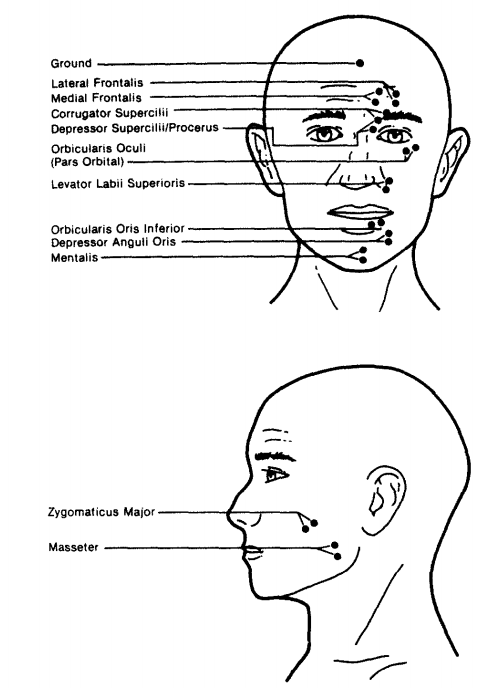
\includegraphics[width=0.9\linewidth]{pictures/Electrodes_placements.png}
  \caption{Atlas of EMG electrode placements for surface differential recording over the major facial mimetic muscles.
}
  \label{fig.background.emg}
\end{figure}
		
		

